% THIS IS SIGPROC-SP.TEX - VERSION 3.1
% WORKS WITH V3.2SP OF ACM_PROC_ARTICLE-SP.CLS
% APRIL 2009
%
% It is an example file showing how to use the 'acm_proc_article-sp.cls' V3.2SP
% LaTeX2e document class file for Conference Proceedings submissions.
% ----------------------------------------------------------------------------------------------------------------
% This .tex file (and associated .cls V3.2SP) *DOES NOT* produce:
%       1) The Permission Statement
%       2) The Conference (location) Info information
%       3) The Copyright Line with ACM data
%       4) Page numbering
% ---------------------------------------------------------------------------------------------------------------
% It is an example which *does* use the .bib file (from which the .bbl file
% is produced).
% REMEMBER HOWEVER: After having produced the .bbl file,
% and prior to final submission,
% you need to 'insert'  your .bbl file into your source .tex file so as to provide
% ONE 'self-contained' source file.
%
% Questions regarding SIGS should be sent to
% Adrienne Griscti ---> griscti@acm.org
%
% Questions/suggestions regarding the guidelines, .tex and .cls files, etc. to
% Gerald Murray ---> murray@hq.acm.org
%
% For tracking purposes - this is V3.1SP - APRIL 2009

\documentclass{acm_proc_article-sp}
\usepackage{url}
\usepackage{hyperref}

\begin{document}

\title{{\ttlit DMD} Project}
\subtitle{Design and implementation of a Publication Management System}
%
% You need the command \numberofauthors to handle the 'placement
% and alignment' of the authors beneath the title.
%
% For aesthetic reasons, we recommend 'three authors at a time'
% i.e. three 'name/affiliation blocks' be placed beneath the title.
%
% NOTE: You are NOT restricted in how many 'rows' of
% "name/affiliations" may appear. We just ask that you restrict
% the number of 'columns' to three.
%
% Because of the available 'opening page real-estate'
% we ask you to refrain from putting more than six authors
% (two rows with three columns) beneath the article title.
% More than six makes the first-page appear very cluttered indeed.
%
% Use the \alignauthor commands to handle the names
% and affiliations for an 'aesthetic maximum' of six authors.
% Add names, affiliations, addresses for
% the seventh etc. author(s) as the argument for the
% \additionalauthors command.
% These 'additional authors' will be output/set for you
% without further effort on your part as the last section in
% the body of your article BEFORE References or any Appendices.

\numberofauthors{3} %  in this sample file, there are a *total*
% of EIGHT authors. SIX appear on the 'first-page' (for formatting
% reasons) and the remaining two appear in the \additionalauthors section.
%
\author{
% You can go ahead and credit any number of authors here,
% e.g. one 'row of three' or two rows (consisting of one row of three
% and a second row of one, two or three).
%
% The command \alignauthor (no curly braces needed) should
% precede each author name, affiliation/snail-mail address and
% e-mail address. Additionally, tag each line of
% affiliation/address with \affaddr, and tag the
% e-mail address with \email.
%
% 1st. author
\alignauthor
Bulat Mukhutdinov\titlenote{Responsible for creation SQL functions, database connection, logger, code optimization}\\
       \affaddr{Innopolis University}\\
       \affaddr{1 Universitetskaya st}\\
       \affaddr{Innopolis, Russia}\\
       \email{bulatmm@yandex.ru}
% 2nd. author
\alignauthor
Timur Shakirov\titlenote{Responsible for creation Web-client, project structure, code optimization, works with the documentation}\\
       \affaddr{Innopolis University}\\
       \affaddr{1 Universitetskaya st}\\
       \affaddr{Innopolis, Russia}\\
       \email{shakirovtr23@gmail.com}
% 3rd. author
\alignauthor Nikolay Yushkevich\titlenote{Responsible for creation XML parser, database structure, works on the data}\\
       \affaddr{Innopolis University}\\
       \affaddr{1 Universitetskaya st}\\
       \affaddr{Innopolis, Russia}\\
       \email{n.yushkevich@hotmail.com}
}
% There's nothing stopping you putting the seventh, eighth, etc.
% author on the opening page (as the 'third row') but we ask,
% for aesthetic reasons that you place these 'additional authors'
% in the \additional authors block, viz.
\date{\normalsize\today}
% Just remember to make sure that the TOTAL number of authors
% is the number that will appear on the first page PLUS the
% number that will appear in the \additionalauthors section.

\maketitle
\begin{abstract}
In this paper we describe the development of the system that is aimed at the management of the publication records. This project is divided into three phases. The first one is designing and implementation of the relational model using an existing DBMS. The second phase is the development of a web based user interface that provides the interaction between user and the database designed in the first phase. The third phase is the development of a new DBMS and the replacement with DBMS used in the first phase.
\end{abstract}

% A category with the (minimum) three required fields
\category{H.4}{Information Systems Applications}{Miscellaneous}
%A category including the fourth, optional field follows...
\category{D.2.8}{Software Engineering}{Metrics}[complexity measures, performance measures]

\terms{Algorithms}

\keywords{DBMS, dblp} % NOT required for Proceedings

\section{Introduction}
The project's aim is to design and implement a publication records management system. In this project we use {\bfseries dblp \cite{dblp}} - Digital Bibliography \& Library Project. It is a computer science bibliography. This source provides an open bibliographic information on major computer science journals and proceedings. It currently contains more than 2.6 million publications with over 1.4 million authors. Moreover, dblp indexes about 25 000 journal volumes, more than 24 000 conferences or workshops, and more than 17 000 monographs.\\
{\bfseries PostgreSQL \cite{postgresql}} is used as a DBMS in order to implement relational model. It is an object-relational database system that can be run on the majority of the operating systems, such as Linux, UNIX (AIX, BSD, HP-UX, SGI IRIX, Mac OS X, Solaris, Tru64), and Windows. Moreover, it has a native programming interface for Java.\\
{\bfseries DbSchema \cite{dbschema}} is used to design the relational model of the project's database and to create database's ER model.
{\bfseries Java \cite{java}} programming language is used for the development of the project.


\section{Phase 1. Design and implementation of the Relational Model}
The aim of this phase is to use the database of different publications for real life problems. As it was mentioned before, dblp bibliography is used to crawl publications data. Therefore, the relational model is based on the structure of dblp. There are 16 entities in it: Article,  Inproceedings, Proceedings, Book, Incollection, Phdthesis, Mastersthesis, www, Article\_author,  Inproceedings\_author, Proceedings\_author,\\ Book\_author, Incollection\_author, Phdthesis\_author, Mastersthesis\_author, www\_author. ER diagram is shown on Figure \ref{fig:ER}. You can see the full size image at \\ \href{https://github.com/BulatMukhutdinov/DMD_Java4Life/blob/master/Report/ER.jpg}{https://github.com/BulatMukhutdinov/DMD\_Java4Life/\\blob/master/Report/ER.jpg}.
\begin{figure}
	\centering
	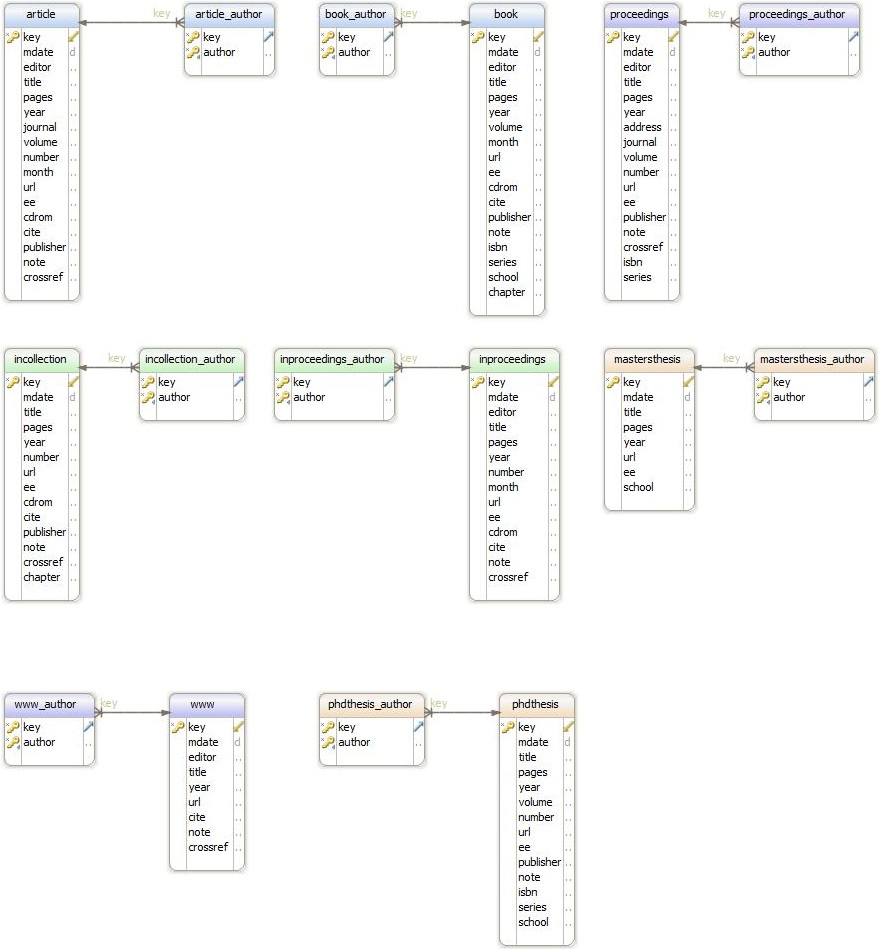
\includegraphics[width=0.7\linewidth]{ER}
	\caption{ER diagram}
	\label{fig:ER}
\end{figure}
\\All publications are connected with their authors as 'one to many'. For example, one Article can have many Article\_authors, one Book can have many Book\_authors and so on. The ER model is based on dblp.dtd and dblp.xml files, that are crawled in real time from \href{http://dblp.uni-trier.de}{http://dblp.uni-trier.de}.
\\
\\The Relations are:
\begin{enumerate}
	\item Article(\underline{key}, mdate, editor, title, pages, year, journal, volume, number, month, url, ee, cdrom, cite, publisher, note, crossref)
	\item Article\_author(\underline{key, author})
	\item Book(\underline{key}, mdate, editor, title, pages, year, volume, month, url, ee, cdrom, cite, publisher, note, isbn, series, school, chapter)
	\item Book\_author(\underline{key, author})
	\item Proceedings(\underline{key}, mdate, editor, title, pages, year, address, journal, volume, number, url, ee, publisher, note, crossref, isbn, series)
	\item Proceedings\_author(\underline{key, author})
	\item Incollection(\underline{key}, mdate, title, pages, year, number, url, ee, cdrom, cite, publisher, note, crossref, chapter)
	\item Incollection\_author(\underline{key, author})
	\item Inproceedings(\underline{key}, mdate, editor, title, pages, year, number, month, url, ee, cdrom, cite, note, crossref)
	\item Inproceedings\_author(\underline{key, author})
	\item Masterthesis(\underline{key}, mdate, title, pages, year, url, ee, school)
	\item Masterthesis\_author(\underline{key, author})
	\item Phdthesis(\underline{key}, mdate, title, pages, year, volume, number, url, ee, publisher, note, isbn, series, school)
	\item Phdthesis\_author(\underline{key, author})
	\item www(\underline{key}, mdate, editor, title, year, url, cite, note, crossref)
	\item www\_author(\underline{key, author})
\end{enumerate}
\subsection{Fillig the database}
After the database structure is created, our XML parser starts to work. This XML parser is based on the standart javax.xml library. Basically, it takes the data from different XML tags and writes them into CSV file, in order to copy this data into our database using COPY FROM command. The COPY FROM command operates much faster than a normal INSERT command because the data is read as a single transaction directly to the target table. On the other hand, it is a very strict format, and the entire COPY procedure will fail if just one line is malformed\cite{copy}.	So our CSV file is accurately created using dblp.xml, all the data has ";" delimiters.
\subsection{Functions}
There are 4 different functions, that were created for Phase 1.
\begin{itemize}
	\item Function that shows all articles that are related to each other by their authors.
	\item Function that shows all articles that are related to each other by their journal.
	\item Function that sorts the 'proceedings' table by 'title' column and returns first 'a\_count' tuple (a\_count is an argument that is equal to 100 by default).
	\item Function that sorts the 'proceedings' table by the count of 'crossref' of table 'article' and returns rows where this count is more or equal to the 'minimal\_count\_of\_crossrefs' argument (minimal\_count\_of\_crossrefs = 10 by default).
\end{itemize}
\subsection{Other technical details}

The project structure is shown on the Figure \ref{fig:ProjectStructure}. 

\begin{figure}[h]
	\centering
	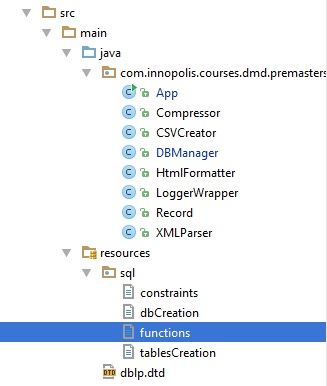
\includegraphics[width=0.7\linewidth]{ProjectStructure}
	\caption{Project structure}
	\label{fig:ProjectStructure}
\end{figure}

The project is divided into 8 classes.
\begin{itemize}
	\item App is a class with a 'main()' method.
	\item Compressor is responsible for zipping and unzipping files.
	\item CSVCreator is responsible for creating CSV files.
	\item DBManager is responsible for the database connection, creating database structure, filling database with data and execution of SQL commands.
	\item HTMLFormatter is responsible for creating HTML document with logs.
	\item LoggerWrapper is responsible for making proper logs.
	\item Record is used in XMLParser for proper data processing.
	\item XMLParser is responsible for parsing dblp.xml file in order to get data from it.
\end{itemize}

\bibliographystyle{unsrt}
\bibliography{sigproc}


\end{document}
